%!TEX encoding = UTF-8 Unicode
\vfill
\pagebreak
\section{Related Work}
\label{sec:RelatedWork}
% Show what you read Start by presenting the structure of component. Show each
% item in a different section. Which works are known as relevant in this area
% Each section should end with a comparative evaluation. End each chapter with a
% synthesis, a table about various solutions, which features are interesting,
% which we want. Finnish sections with a work summary on a single sentence.

The solution proposed in this document leverages knowledge obtained from studying several concepts and systems from the current state-of-the-art. In this section, an overview of those concepts and systems will be given, stating for each of them their advantages and disadvantages. This section is structured as follows. Section \ref{sec:Computingparadigms} presents different methods to push intelligence and computing power closer to the source of the data and why this work adopted fog computing for this purpose. Section \ref{sec:Mobility} presents mobility-aware systems xxx. Section \ref{sec:Dataplacement} xxx. \ref{sec:Migration} xxx. \ref{sec:Multiobjective} xxx. Section \ref{sec:Toolkits} xxx.

%!TEX encoding = UTF-8 Unicode
\subsection{Related computing paradigms}
\label{sec:Computingparadigms}
In what concerns about standardizing fog computing, there is a lack of unanimity. As aforementioned, fog has been variously termed as cloudlets, edge computing, etc. Different research teams are proposing many independent definitions of fog (and fog-related computing paradigms). As there is a research gap in the definitions and standards for fog computing, this work follows the definitions that Ashkan Yousefpour et al. \cite{yousefpour2018all} present. Below, are described some paradigms that were raised in order to bring cloud closer to the end devices, as well as their pros and cons. As a conclusion we show why fog computing is the natural platform for IoT.

\subsubsection{Mobile Computing}\label{subsec:MC}
Mobile/nomadic computing (MC) is characterized by the processing being performed by mobile devices (e.g., laptops, tablets, or mobile phones). It raises to overcome the inherent limitations of environments where connectivity is sparse or intermittent and where there is low computing power. As this model only uses mobile devices to provide services to clients, there is no need for extra hardware. They already have communication modules such as Bluetooth, WiFi, ZigBee, etc. As already mentioned, mobile devices have evolved in recent years. However, their resources are more restricted, compared to fog and cloud. This computing paradigm has the advantage of being characterized by a distributed architecture, once mobile machines do not need a centralized location to operate. The disadvantages of MC are mainly due to their hardware nature (i.e. low resources, balancing between autonomy and the dependency of other mobile devices; characteristic that prevails in all distributed architectures) and the need of mobile clients to efficiently adapt to changing environments \cite{satyanarayanan1996fundamental}. MC alone may not be able to meet the requirements of some applications. It is limited on the one hand due to autonomy constraints and in the order hand by low computational and storage capacity. This restricts the applications where this paradigm is feasible. For instance, it is unsuitable for applications that require low-latency and that, at the same time, generate large amounts of data that needs to be stored or processed. Nonetheless, MC can use both fog and cloud computing to enhance its capacities, not being restricted to a local network; expanding the scope of mobile computing and the number of applications where it can be used.

\subsubsection{Mobile Cloud Computing}
Cloud and fog computing, as mentioned in \ref{subsec:MC}, are key elements for validate the importance of MC. This interaction between them results in a new paradigm, called mobile cloud computing (MCC). MCC, differs from MC in the sense that mobile applications can be partitioned at runtime so that computationally intensive components of the application can be handled through adaptive offloading \cite{shiraz2013review}, from mobile devices to the cloud. This characteristic increases the autonomy of mobile devices (i.e battery lifetime), as both the data storage and data processing may occur outside them. Also, it enables a much broader range of mobile subscribers, rather than the previous laptops, tablets, or mobile phones. Opposed to resource-constrained in MC, MCC has high availability of computing resources, scaling the type of applications where it is possible to use (e.g., augmented reality applications). Unlike MC, MCC relies on cloud-based services, where its access is done through the network core by WAN connection, which means that applications running on these platforms require connection to the Internet all the time. On the one hand, both MCC and MC suffer from the intrinsic characteristics of mobility, such as frequent variations of network conditions (intensified under rapid mobility patterns), and on the other hand, in MCC, even if the mobile devices remain fixed, it suffers from the inherent disadvantage of using cloud-based services (i.e. communication latency), which makes it unsuitable for some delay-sensitive applications with heavy processing and high data rate.

\subsubsection{Mobile ad hoc Cloud Computing}
In some scenarios there exists lack of infrastructure or a centralized cloud, so implement a network based on MCC may not always be suitable. To overcome dependence on an infrastructure, raises mobile ad hoc cloud computing (MACC). It consists on a set of mobile nodes that form a dynamic and temporary network through routing and transport protocols. These nodes are composed by mobile ad hoc devices which may continuously join or leave the network. In order to counteract the aforementioned characteristics inherent to this type of networks, and unlike MC, a set of ad hoc devices may form a local cloud that can be used in the network for purposes of storage and computation. As mobile ad hoc networks (MANET), it is imperative in use cases such as disaster recovery, car-to-car communication, factory floor automation, unmanned vehicular systems, etc. Although it does not rely on external cloud-based services as MCC does, which mitigates the latency problem, it shares some limitations inherent to MC and ad hoc networks such as the power consumption constraints. Moreover, the formed local cloud may still be computationally weak and, as both network and cloud are dynamic it is more challenging to achieve an optimal performance (i.e. as there is no infrastructure, mobile devices are also responsible for routing traffic among themselves).

\subsubsection{Edge Computing}
Edge computing (EC), makes use of connected devices at the edge of the network to enhance its capabilities (i.e. management, storage, and processing power). It is located in the local IoT network, being ideally at one hop away from the Iot device and at most located few hops away. Open Edge Computing defines EC as computation paradigm that provides small data centers (edge nodes) in proximity to the users, enabling a dramatic improvement in customer experience through low latency interaction with compute and storage resources just one hop away from the user \cite{OpenEdge73:online}. As in EC the connected devices don't have to wait for a centralized platform to provide the requested service, nor are so limited in terms of resources as in the traditional MC, their service availability is relatively high. Also, the restrictions over the autonomy are not so tight once there are not only mobile devices. Nonetheless, EC has some drawbacks. As latency, in this context, is composed by three components: data sending time, processing time and result receiving time, even though the communication latency is negligible, processing time may not be. This computing paradigm only uses edge devices, and their computation and storage power may still be poor (e.g., routers, switches), compared to fog or cloud computing, so this processing latency may still be too high for some applications.\\
\noindent\tab OpenFog Consortium states that fog computing is often erroneously called edge computing, but there are key differences between the two concepts \cite{OpenFog0208}. Although they have similar concepts, edge computing tends to be limited to the edge devices (i.e. located in the IoT node network), excluding the cloud from its architecture. Whereas, fog computing is hierarchical and unlike EC, it is not limited to a local network, but instead it provides services anywhere from cloud to things. It is worth noting that the term edge used by the telecommunication's industry usually refers to 4G/5G base stations, radio access networks (RANs), and internet service provider (ISP) access/edge networks. Yet, the term edge that is recently used in the IoT landscape refers to the local network where sensors and IoT devices are located \cite{yousefpour2018all}.

\subsubsection{Multi-access Edge Computing}
Analogously, MCC is an extension of MC through CC, as multi-access edge computing (MEC) is an extension of MC through EC (telecommunication industry definition). ETSI defines MEC as computation paradigm that offers application developers and content providers cloud-computing capabilities and an IT service environment at the edge of the network. This environment is characterized by ultra-low latency and high bandwidth as well as real-time access to radio network, information that can be leveraged by applications \cite{ETSIMult81:online}. In MEC, operators can open their RAN edge to authorized third parties, allowing them to deploy applications and services towards mobile subscribers through 4G/5G base stations. The first approach to the edge of a network meant the edge of a mobile network, hence the name mobile edge computing. As MEC research progressed, was noticed that the term leaves out several access points that may also construct the edge of a network. Thus, prompted the change from mobile edge computing to multi-access computing in order to reflect that the edge is not solely based on mobile networks \cite{MobileEd74:online}. Now it includes a broader range of applications beyond mobile device-specific tasks, such as video analytics, connected vehicles, health monitoring, augmented reality, etc. Similar to EC, MEC can operate with little to no Internet connectivity and use small-scale data centers with virtualization capacity to provide services. MEC is expected to benefit significantly from the up-and-coming 5G platform as it allows for lower latency and higher bandwidth among mobile devices, and it supports a wide range of mobile devices with finer granularity.\\
\noindent\tab Both fog computing and MEC have the objective of offering similar type of features. Fog computing concentrates on applications, mainly IoT, that take advantage of a platform set that collectively assist end devices. MEC, on the other hand, focuses on application-related enhancements in terms of feedback mechanisms, information and content processing and storage, etc \cite{taleb2017multi}.

\subsubsection{Cloudlet Computing}
Cloudlet computing is another direction in mobile computing that aims to bring cloud closer to end devices through the use of cloudlets. M. Satyanarayanan et al. states that a cloudlet is a trusted, resource-rich computer or cluster of computers that's well-connected to the Internet and available for use by nearby mobile devices \cite{satyanarayanan2009case}. Cloudlet is, as the name suggests, a smaller sized clouds with lower computational capacity. It can be seen as a ``data center in a box'', where mobile users can exploit their virtual machines (VM) to rapidly instantiate customized-service software in a thin client fashion. This way, it is possible to offload computation from mobile devices to VM-based cloudlets located on the network edge (telecommunication industry definition). Through those VMs, cloudlets are capable of providing resources to end devices in real-time over a WLAN network. The relatively low hardware footprint, results in moderate computing resources, but lower latency and energy consumption and higher bandwidth compared to cloud computing. The characteristics of this computing paradigm make possible to handle applications with low-latency requirements, supporting real-time IoT applications. Y Jararweh et al. \cite{jararweh2013resource} propose an architecture mobile-cloudlet-cloud, where they present three reasons which indicate that even though cloudlets are computationally powerful, they still need a connection to the cloud and its services: (1) Heavy non real time jobs might process in the enterprise cloud whiles the real-time ones processed by the cloudlet, (2) Accessing a file stored in the Enterprise Cloud, (3) Accessing some services that are not available inside the Cloudlet. Although cloudlet computing fits well with the mobile-cloudlet-cloud architecture, fog computing offers a more generic alternative that natively supports large amounts of traffic, and allows resources to be anywhere along the cloud-to-things continuum. As it will be shown later, cloudlets are great resources and, in this way, they can be combined with the fog computing paradigm.

%muita coisa copiada, tentar reescrever
\subsubsection{Mist Computing}
Mist computing emerges to push IoT analytics to the extreme edge. This computing paradigm is an even more dispersed version of fog. That means locating analytics tools not just in the core and edge, but at the ``extreme edge'' \cite{Ciscopus95:online}. Mist computing layer is composed by mist nodes that are perceived as lightweight fog nodes. They are more specialized and dedicated nodes with low computational resources (e.g., microcomputers, microcontrollers) that are even closer to the end devices than the fog nodes \cite{iorga2018fog}. Therefore, mist computing can be seen as the first (non-mandatory) layer in the IoT-fog-cloud continuum. It extends compute, storage, and networking across the fog through the \textit{things}. This decreases latency and increases subsystems' autonomy. It can be implemented in order to enhance the services of predominance of wireless access and mobility support. The challenge with implementing mist computing systems lies in the complexity and interactions of the resulting network. These must be managed by the devices themselves as central management of such systems is not feasible.

\subsubsection{Concluding Remarks}
Just like the above-mentioned, there are some other similar computing paradigms such as follow me cloud (FMC), follow me edge (FME), follow me edge-cloud (FMeC) and cloud of things (CoT), to name a few. However, this state-of-the-art had as first objective to investigate the most relevant and treated ones in the literature. The purpose was to understand their characteristics and identify where to tackle the current limitations which oppose the deployment of delay-sensitive IoT systems in mobile environments. Fig. \ref{computing_paradigms} shows a classification of the these paradigms and their overlap in terms of their scope.\\
\noindent\tab As shown with the attributed pros and cons to these computing paradigms, they all have been proposed to cover different use cases. Even so, fog computing is suited for many use cases, including data-driven computing and low-latency applications, being the most versatile and comprehensive one. As aforementioned, fog is flexible enough to interact and take advantage of other paradigms such as edge, cloud, cloudlet and mist computing. Nonetheless, it may not be suitable for a few extreme use cases, such as disaster zones or sparse network topologies where ad hoc computing (e.g., MACC) may be a better fit.
\begin{figure}[t]
	\centering
	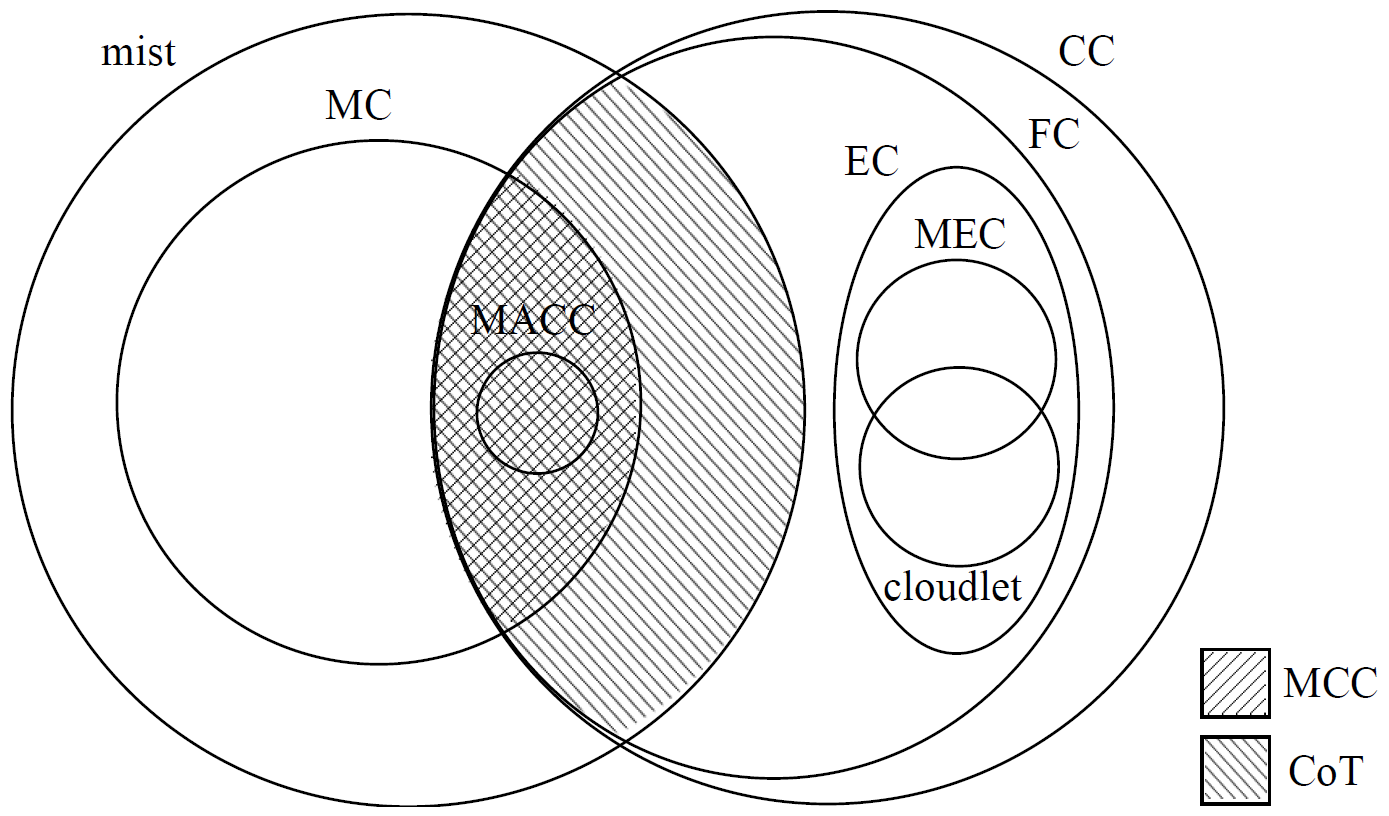
\includegraphics[width=90mm]{images/computing_paradigms}
	\caption{A classification of scope of fog computing and its related computing paradigms.\protect\footnotemark}
	\label{computing_paradigms}
\end{figure}
\footnotetext{Figure adapted from \cite{yousefpour2018all}.}
%!TEX encoding = UTF-8 Unicode
\subsection{Fog computing architecture}
Fog computing is a great resource to support IoT applications' requirements. Taking into account what has been mentioned in Section \ref{sec:Introduction} and Section \ref{sec:Computingparadigms}, fog computing has, the below, eight fundamental characteristics which validate the statement uttered above \cite{iorga2018fog}:
\begin{itemize}
	\item \textbf{Contextual location awareness, and low latency}. Provides low latency due to the proximity between the IoT devices and the fog nodes. Also, the contextual location allows them to be aware of the cost of communication latency with both other fog nodes and the end devices, allowing the distribution of applications across the network to be organized in a weighted manner;
	\item \textbf{Geographical distribution}. Uses anything between the cloud and \textit{things} to provide ubiquitous computing, allowing continuity of service in mobile environments;
	\item \textbf{Heterogeneity}. Supports wide diversity of communications, applications and services;
	\item \textbf{Interoperability and federation}. Uses cooperation of different providers to support heavy applications such as real-time streaming. Moreover, it supports migration of applications to more suited fog servers depending on the current context;
	\item \textbf{Real-time interactions}. Applications may involve real-time interactions rather than batch processing (e.g., as cloud does);
	\item \textbf{Scalability and agility of federated, fog-node clusters}. Fog is adaptive; may form clusters-of-nodes or cluster-of-clusters to support elastic compute, resource pooling, etc;
	\item \textbf{Predominance of wireless access}. Most of the end devices only support wireless communication;
	\item \textbf{Support for mobility}. The exponential growth of mobile devices demands mobility support.
\end{itemize}

Nonetheless, fog still has some limitations (as stated in Section \ref{subsec:Objectives}). In order to tackle those limitations, first it is needed an overview over its architecture. This includes understanding what are the actors and how they interact, how IoT nodes connect to the fog servers, how clients outsource the allocation and management of resources that they rely upon to these servers, how the location-aware and migration features are performed, etc.

\subsubsection{Overview}
\noindent\tab Fog computing is composed by fog nodes/servers, that allow the deployment of distributed, latency-aware applications and services. Those nodes can be either virtual (e.g., gateways, switches, routers, servers) or physical (e.g., virtualized switches, virtual machines, cloudlets) components that provide computing resources to end devices. They can be organized in clusters either vertically (to support isolation), horizontally (to support federation), or relative to fog nodes’ latency-distance to the IoT devices \cite{iorga2018fog}. Fog nodes can be accessed through connected devices located at the edge, which provide local computing resources and, when needed, provide network connectivity to centralized services (i.e. cloud). Moreover, fog nodes can operate in a centralized or decentralized manner and can be configured as stand-alone nodes.\\
\noindent\tab Fig. \ref{fog_architecture} shows the typical fog computing architecture. As stated before, mist computing can be implemented in a layer between the fog servers and the end devices. Moreover, the presence of cloud servers is not imperative, however it is very important for numerous applications.
\begin{figure} [t]
	\centering
	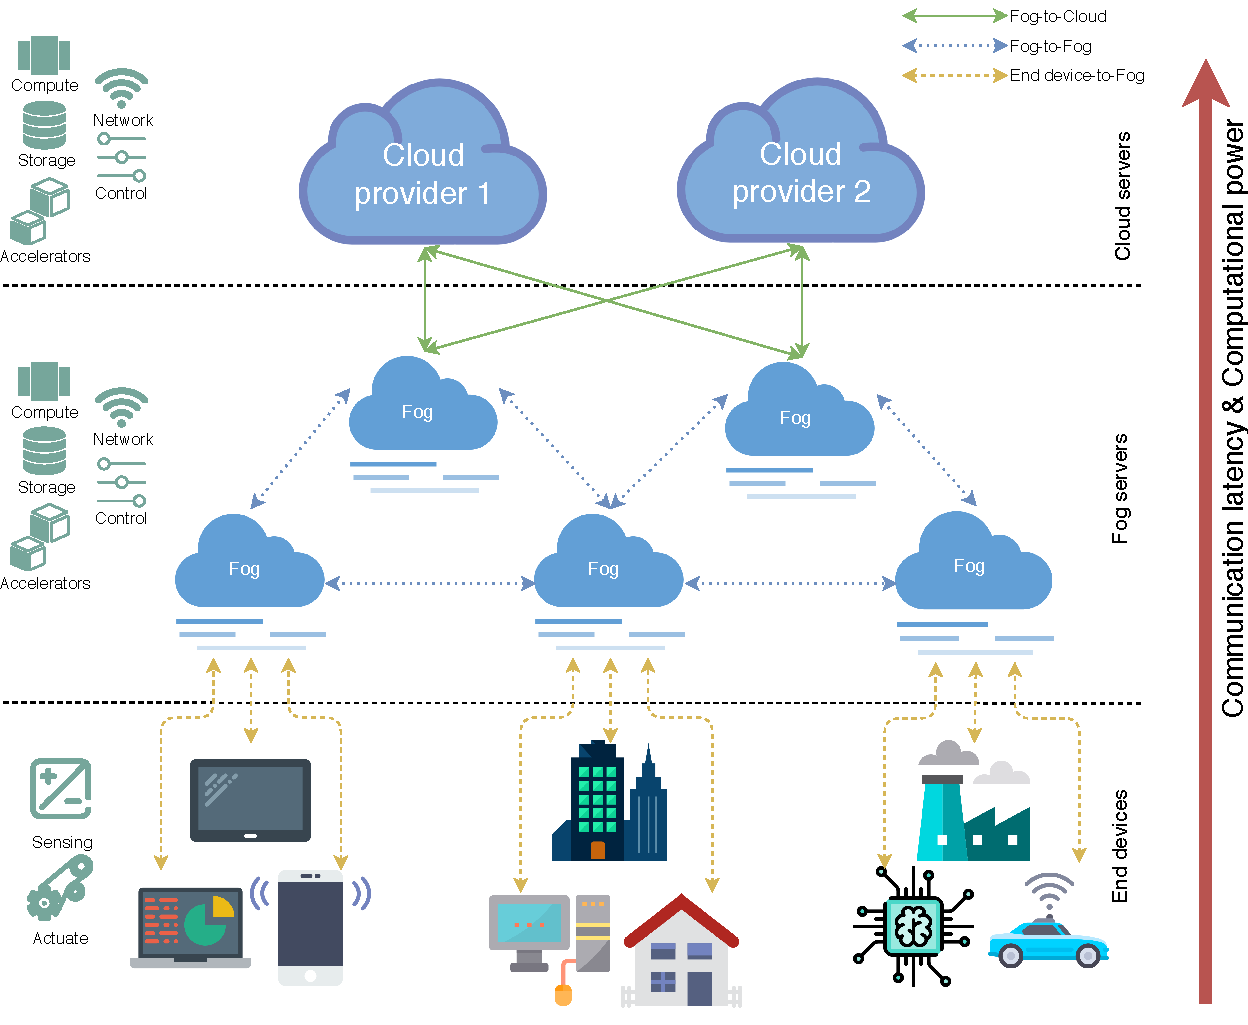
\includegraphics[width=0.9\textwidth]{images/fog_architecture/fog_architecture}
	\caption{Typical architecture of fog computing.}
	\label{fog_architecture}
\end{figure}
It is worth noting that, once fog nodes can be anything with computational and storage power in the cloud-to-things continuum, the links formed in these architectures (i.e. End device-to-Fog, Fog-to-Fog and Fog-to-Cloud) can be of any type. For instance, end devices can be connected to fog servers by wireless access technologies (e.g., WLAN, WiFi, 3G, 4G, ZigBee, Bluetooth) or wired connection. Moreover, fog nodes can be interconnected by wired or wireless communication technologies and they can be linked into the cloud by IP core network. Nonetheless, in order to provide location awareness, the fog layer also needs Location-Based Services (LBSs) that provide location information.

\noindent\tab In this architecture, the connected sensors located at the edge, generate data that can adopt two models. First, in a sense-process-actuate model, the information collected is transmitted as data streams, which is acted upon by applications running on fog devices and the resultant commands are sent to actuators. In this model, the raw data collected often does not need to be transferred to the cloud; data can be processed, filtered, or aggregated in fog nodes, producing reduced data sets. The result can then be stored inside fog nodes or actuated upon through the actuators. Second, in a stream-processing model, sensors send equally data streams, where the information mined (from the incoming streams) is stored in data centers for large-scale and long-term analytics. In this case, big data needs to be stored and does not have that much latency constraints. Being fog servers less powerful than the cloud ones, cloud is far more suited for this kind of operations. Yet, fog servers can still shrink data, doing some intermediate processing as in the previous model. This meets the aforementioned statement - although cloud is not essential for the functioning of fog, in some applications it is beneficial or even essential.\\
\noindent\tab Fog servers are the fundamental components in this three tier architecture (i.e. IoT-fog-cloud). They are able to support the six features shown below \cite{iorga2018fog}:
\begin{itemize}
	\item \textbf{Autonomy}. Fog nodes can be autonomous enough to operate independently, making local decisions, at the node or cluster-of-nodes level;
	\item \textbf{Heterogeneity}. Can be deployed in a wide variety of environments;
	\item \textbf{Hierarchical clustering}. The fog network can be organized with different numbers of layers, so that they are able to provide different subsets of service functions while working together as a continuum;
	\item \textbf{Manageability}. They are managed and orchestrated by complex systems that can perform most routine operations automatically;
	\item \textbf{Programmability}. Fog nodes are inherently programmable at multiple levels, by multiple stakeholders such as network operators, domain experts, equipment providers, or end users.
\end{itemize}
\noindent\tab Fog nodes generally are of most value in scenarios where data needs to be collected at the edge and where the data from thousands or even millions of devices is analyzed and acted upon in micro and milliseconds \cite{openfog2017openfog}. In order to being able to support such a large number of requests, especially those engaged in enhanced analytics, fog nodes may implement additional hardware. Accelerators modules (refer to Fig. \ref{fog_architecture}) can be implemented to provide supplementary computational throughput. For instance, hardware accelerators can be performed through Graphics Processing Unit (GPUs); they are an optimal choice for applications that support parallelism or for stream processing. Also, fog nodes can opt to make use of Field Programmable Gate Arrays (FPGAs) or even Digital Signal Processors (DSPs) for this propose.
%verificar gateways no Assessment of the Suitability of Fog Computing in the Context of Internet of Things
\subsubsection{Data Placement}

\noindent\tab Moreover, the applications deployed by the end users in fog nodes can be seen either as a whole or as a distributed data flow (DDF) model, in which the applications are moduled as a collection of modules. This can be particular useful so that the less restricted modules in terms of latency can be deployed to the upper fog layers (ideally to the cloud), leaving the fog nodes of the lower layers less overloaded, being able to respond faster to modules within tighter latency bounds. Nonetheless, fog nodes can communicate between them to perform data and process management in order to support application requirements, as well as to exchange fog control/management data such as user device and application state.\\

\subsubsection{Virtualization Mechanisms}

In general, hosting an application involves creating a set of virtual machines (VMs) or execution containers (e.g., Docker) and assigning them a vector of computing resources (such as CPU, memory and storage) from the physical machines (PMs) in the edge-cloud.

\subsubsection{Orchestration}
\noindent\tab When an end device needs to offload some work to a third party, it needs somehow to know where to outsource the allocation and management of resources that they rely upon. For this propose, the fog architecture also needs a discovery and orchestration service which concerns in finding the best available fog server, given certain capabilities and requirements.\\

\noindent\tab In this context, E Saurez et al. \cite{saurez2016incremental} propose foglets, a programming model that facilitates distributed programming across fog nodes. Foglets are implemented in fog nodes using container technology. They provide APIs for app development as a dataflow graph whose nodes can be placed in the different levels of the computational hierarchy. In additional to the provided primitives for communication between the application components, it also embodies algorithms for the discovery and incremental deployment of resources commensurate with the application needs. Moreover it provides mechanisms for QoS-sensitive and workload sensitive migration of application components due to end devices mobility and application dynamism. Specifically they show that there are four entities in the foglets runtime system: the discovery server, the docker registry server, the entry point daemon, and finally the worker process. The discovery server is a partitioned name server that maintains a list of fog nodes available. Docker registry server is a server that contains the binaries for the applications that have been launched on the foglets infrastructure. The entry point daemon executes directly on top of the host OS in the fog node, awaits requests and periodically sends ``I am alive'' message to the discovery server. Finally the worker process that will carry out the functionality contained in a particular application component assigned to it.\\

\noindent\tab Also in this context, F Bonomi et al. \cite{bonomi2014fog} propose a fog computing layer architecture that is classified into two sub-layers: (1) the fog abstraction layer, and (2) the fog orchestration layer. While the former enables virtualization, provides data and resource isolation guarantees, manages the fog resources, and preserves security and privacy, the latter provides dynamic, policy-based life-cycle management of fog services. The fog orchestration layer comprises of a software agent, Foglet, with reasonably small footprint yet capable of bearing the orchestration functionality and performance requirements. Moreover, this layer also needs a distributed, persistent storage to store policies and resource meta-data (e.g., capability, performance) that support high transaction rate update and retrieval, a scalable messaging bus to carry control messages for service orchestration and resource management and finally a distributed policy engine with a single global view and local enforcement.\\

\noindent\tab Julien Gedeon \cite{gedeon2017router}, propose a brokering mechanism in which available surrogates (e.g., cloudlets) advertise themselves to the broker. The broker receives client requests and considers a number of attributes such as network information, hardware capabilities, and distance to find the best available surrogate for the client. They look at the problem of surrogate discovery in the context of an urban area, where they are faced with a high mobility of end devices. Multiple brokers are interconnected using Distributed Hash Tables (DHTs) in order to exchange information.\\

%Applications that require characteristics such as low latency, geo-distribution, mobility, high resilience, and large-scale distributed systems benefit from the Fog.
%\noindent\tab Similar to the traditional cloud computing, fog offers tree types of service models: Software as a Service (SaaS), Platform as a Service (PaaS) and Infrastructure as a Service (IaaS).
\noindent\tab Fog servers can provide reduced latencies and help in avoiding/reducing traffic congestion in the network core. However, this comes at a price: more complex and sophisticated resource management mechanisms are needed. This raises new challenges to be overcome such as dynamically deciding when, and where (device/fog/cloud) to carry out processing of requests to meet their QoS requirements. Furthermore, in mobile environments such mechanisms must incorporate mobility (i.e. location) of data sources, sinks and fog servers in the resource management and allocation process policies to promote and take advantage of proximity between fog and users.
%!TEX encoding = UTF-8 Unicode
\subsection{Data placement}
\label{sec:Data_placement}

\cite{li2018virtual}
They propose a layered Fog framework to better support IoT applications through virtualization. The virtualization is divided into object virtualization  (VOs), network function virtualization and service virtualization. VOs to address the protocol inconsistency (lack of unified networking protocols that leads to exaggerated overhead); Network function virtualization maps standard networking services to VOs, thus, minimize the communication process between consumers and producers by minimizing latency, improving security and scalability; Service virtualization that composes the community and Cloud Apps from various vendors to serve local Fog users with high quality of experience (QoE) but at low cost. At last, Foglets are involved to seamless aggregate multiple independent virtual instances, Fog network infrastructures, and software platforms.\\

\cite{giang2015developing}
This paper proposes a Distributed Dataflow (DDF) programming model for the IoT that utilizes computing infrastructures across the Fog and the Cloud. Also, evaluate their proposal by implementing a DDF framework based on Node-RED (Distributed Node-RED or D-NR), a visual programming tool that uses a flow-based model for building IoT applications. To address challenges of the intrinsic nature of the IoT (heterogeneous devices/resources, a tightly coupled perception-action cycle and widely distributed devices and processing), they propose a Distributed Dataflow (DDF) programming model for the IoT that utilities computing infrastructures across the Fog and the Cloud. Also, they evaluate their proposal by implementing a DDF framework based on Node-RED (Distributed Node-RED or D-NR), a visual programming tool that uses a flow-based model for building IoT applications.\\

\cite{bahreini2017efficient}
The authors address the problem of multi-component application placement on fog nodes. Each application could be modeled as a graph, where each node is a component of the application, and the edges indicate the communication between them.\\


\cite{bruschi2018move}
With the state-of-the-art virtualization technologies, services can be implemented in modular software as a graph/chain of portable VOs that can be dynamically migrated around the Telco infrastructure. It is proposed a VO clustering and migration policy that jointly considers user proximity and inter-VO affinity to scalably support user mobility, while allowing service differentiation among users.\\
%\subsubsection{Virtual Objects} \label{subsec:VirtualObjects}
%\subsubsection{Virtual Machines} \label{subsec:VirtualMachines}
%!TEX encoding = UTF-8 Unicode
\subsection{Migration optimization in mobile fog environments}
\label{sec:Migration}
When an IoT device needs to offload some heavy application to a third party, it will be connected to the nearest server, securing an one-hop away fog server to ensure the shortest network delay. However, as their physical distance increases either by device or server movement, their network distance (i.e. the number of hops) will also increase. Hence, both latency and bandwidth usage by the intermediate links will increase, resulting in poor connectivity. This away, in such dynamic environments the decision-making of where to send the VMs, in order to overcome these limitations, is a major concern. Moreover, even if both clients and servers are static, the end-to-end latency may increase due to unexpected crowds of mobile clients seeking to connect or making requests to the same fog server simultaneously.\\
\noindent\tab In Section \ref{sec:Dataplacement} was verified that applications can be offloaded as a whole, or as a set of modules that may have different constraints. Regardless of their type, whenever it is justified the system needs to be readjusted. This is performed through the exchange of VMs (that contain the applications or modules) between fog nodes. For this reason, it is necessary to answer the following two questions: \textit{When is this exchange justified? And what is the best placement for those applications and/or modules?}\\

%%Previous reactive load balancing algorithms migrate VMs upon the occurrence of load imbalance, while previous proactive load balancing algorithms predict PM overload to conduct VM migration
% another works were performd using MDP-based approaches (ex. Distributed Autonomous Virtual Resource Management in Datacenters Using Finite-Markov Decision Process)

\subsubsection{Latency-aware with mobile end-devices}
\noindent\tab In the context of mobile end devices, B Ottenwälder et al. \cite{ottenwalder2013migcep} state that as sensors and consumers are mobile, the latency (between the access point of a mobile sensor and the fog node) and bandwidth usage is expected to change over time, so it is necessary to constantly adapt the placement through migrations to new fog nodes. However, each migration comes with a cost; consequence of the local state that also needs to be migrated. Thus, frequent migration would significantly decrease the system performance. To overcome this limitation, they propose a placement and migration method for providers of infrastructures that incorporate cloud and fog resources to support operator migrations in mobile complex event processing (MCEP) systems. Their method plans the migration ahead of time through knowledge of the MCEP system and predicted mobility patterns towards ensuring application-defined end-to-end latency restrictions and reducing the network utilization. These predicted mobility patterns were captured using three different methods: uncertain locations from the \textit{dead reckoning} approach (linear), certain locations that could stem from a \textit{navigation} system (navi), and \textit{learned} transitions between leaf broker (learned). This method, allows a minimization of migration costs by selecting migration targets that ensure a low expected network utilization for a sufficiently long time. Moreover, they present how the application knowledge of the CEP system can be used to improve current live migration techniques for VMs to reduce the required bandwidth during the migration (i.e. unnecessary events are not migrated).\\

\noindent\tab A different approach was adopted in the work of R Urgaonkar et al. \cite{urgaonkar2015dynamic}. Similarly to the previous work, their aim is to provide an optimal decision with regard to: where to migrate a current service as the user location changes. However, they argue that because of the uncertainty in user mobility and request patterns, it is challenging to make the decision in an optimal manner. Also, in this work is argued that methods that depend on mobility patterns have several drawback, namely: (1) it requires extensive knowledge of the statistics of the user mobility and request arrival processes that can be impractical to obtain in a dynamic network, (2) even when this is known, the resulting problem can be computationally challenging to solve, and (3) any change in the statistics would make the previous solution suboptimal and would require recomputing the optimal solution. Thus, they propose a new model, inspired by the technique of Lyapunov optimization, that overcomes these drawbacks (i.e. does not require any knowledge of the transition probabilities). The overall problem of dynamic service migration and workload scheduling to optimize system cost while providing end user performance guarantees is formulated as a sequential decision making problem in the framework of markov decision problems (MDPs). However, they have developed a new approach for solving a class of constrained MDPs that possess a decoupling property. When this property holds, their approach enables the design of simple online control algorithms that do not require any knowledge of the underlying statistics of the MDPs.\\
%This technique was applied to both dynamic service migration and workload scheduling and compared to three other policies: never migrate policy, always migrate policy and myopic policy (recalculate the system parameters in time slots). \\

\noindent\tab W Zhang et al. \cite{zhang2016segue} state that previous studies have proposed a static distance-based MDP for optimizing migration decisions. However, these models fail to consider dynamic network and server states in migration decisions, assuming that all the important variables are known. Moreover, they also point out another unaddressed problem which lies in the recalculation time interval of the method. Since running MPD is a heavy computing task, a short recalculation interval introduces a considerable overhead to the server. On the other hand, a long recalculation interval may translate into lazy migration, meaning that resulting in periods of transgression of QoS guarantees. In order to overcome those issues, the authors propose SEGUE. This model achieves optimal migration decisions by providing a long-term optimal QoS to mobile users in the presence of link quality and server load variation. Additionally, SEGUE adopts a QoS aware scheme to activate the MDP model. In other words, it only activates the MDP model when QoS violation is predicted. Thus, it avoids unnecessary migration costs and bypass any possible QoS violations while keeping a reasonable low overhead in the servers.\\

\noindent\tab The work performed by Wuyang Zhang et al. \cite{Zhang2017} use as case study the Massively Multiplayer Online Gamse (MMOGs) with Virtual Reality (VR) technologies, VR-MMOGs. They present the main challages of VR-MMOGs, namely: stringent latency, high bandwidth, and large scale requirements. This work shows one problem that remains unsolved: how to distribute the work among the user device, the edge clouds, and the center cloud to meet all three requirements especially when users are mobile. Their approach was to place local view change updates on edge clouds for immediate responses, frame rendering on edge clouds for high bandwidth, and global game state updates on the center cloud for user scalability. In this kind of games, the users need to move, so in order to keep a low latency communication, they also ropose an efficient service placement algorithm based on MDP. This method takes into account the presence of dynamic network states and server workload states, and user mobility. To ensure feasibility of this method, they come up with an approach that reduces the algorithm complexity in both storage and execution time. Nonetheless, unlike many of the service migration solutions which assumes an ignorable service transition time, they point out that it is impossible to migrate an edge service from one edge to another instantly given the size of a VR game world. Therefore, they propose a mechanism to ensure a new edge cloud is activated when a player connects to the new one.\\

\noindent\tab S Abdelwahab et al. \cite{abdelwahab2018clones} argue that IoT devices communicate a large number of messages with many devices. Thus, devices with low computing and storage capacities will became another source of latency for large-scale distributed applications. Their experiments show that brokering the messages through a one-hop away broker may reduce significantly the end-to-end latency. Therefore, if devices are cloned in a one-hop away cloudlet, their clones can provide message brokering service, allowing both a communication with minimal latency between devices and to offload intensive computation into rich memory and processing nodes that host the clones. Nonetheless, communicating through a one-hop away clone may still experience long end-to-end latency when the broker service relays messages to distant devices. Hence, they propose FogMQ, a self-deploying brokering clones that discover hosting platforms and autonomously migrate between them according to the measured end-to-end latency. This method does not need a central monitoring and control unit. FogMQ servers expose tomography functionalities that enables clones to take migration decisions without complete knowledge about the hosting platform. It allows to stabilize clones deployment and achieve a near minimum latency given an existing infrastructure limits.\\

\noindent\tab The study performed by X Sun et al. \cite{sun2016primal} presents, similarly to the previous ones, a case scenario where end devices are mobile. To preform this work they use a cloudlet network architecture to bring the computing resources from the centralized cloud to the edge. They present the PRofIt Maximization Avatar pLacement (PRIMAL) strategy. PRIMAL maximizes the trade-off between the migration gain (i.e. the end-to-end delay reduction) and the migration cost (i.e. the migration overheads), selectively migrating the avatars (an application clone located in a cloudlet) to their optimal locations.\\ %Does not address where this strategy is calculated and the time interval (verificar melhor).

\noindent\tab 

\subsubsection{Latency-aware with mobile fog servers}
D Ye et al. \cite{ye2016scalable} leverage the characteristics of buses and propose a scalable fog computing paradigm with servicing offloading in bus networks. Knowing that buses have fixed mobility trajectories and strong periodicity, they consider a fog computing paradigm with service offloading in bus networks which is composed by two parts: roadside cloudlets and bus fog servers. The roadside cloudlet consists of three components: dedicated local servers, location-based service (LBS) providers, access points (APs). The dedicated local servers virtualize physical resource and act as a potential cloud computing site. The LBS providers offer the real time location of each bus in bus networks. The APs act as gateways for mobile users and bus fog servers within the communication coverage to access the roadside cloudlet. When users need to offload some computationally intensive and delay sensitive tasks, they access APs and use the computing service of the roadside cloudlet. However, as cloudlets have limited computational and storage resources, they may became overloaded. The bus fog server is a virtualized computing system on bus, which is similar to a light-weight cloudlet server. Hence, those buses not only provide fog computing services for the mobile users on bus, but also are motivated to accomplish the computation tasks offloaded by roadside cloudlets. This allocation strategy is accomplished using genetic algorithm (GA), where the objective is to minimize the cost that roadside cloudlets spend to offload their computation tasks. Meanwhile, the user experience of mobile users are maintained. Although this work refers to mobile users, its meaning is not literal, being supported only the mobility of fog servers. In their problem formulation there are two types of mobile users. On one hand there are mobile users that already have offloaded their computing tasks to the roadside cloudlets (i.e. representing the workload of the cloudlets). On the other hand there are several mobile users inside the bus that have also offloadded their tasks (i.e. representing the workload of bus fog servers).%foi em que simulador?


%There are two possibilities to answer the question: \textit{when is this exchange justified?}
%In both, it is necessary to monitor the relevant system parameters, however in a different way. The first is to 

\subsection{Mobile Fog Computing}
\label{sec:Mobility}
The concept of mobile fog computing is similar to fog computing, in which both IoT and fog nodes are mobile components. Those are connected wirelessly (e.g., via WiFi or Bluetooth). The challenge with implementing fog computing in mobile environments lies in the underlying complexity of data placement management and decision-making to ensure the QoS to all users (i.e. ensure that all latency constraints of users' applications are met).\\

In this context, Luiz F. Bittencourt et al. \cite{bittencourt2017mobility} took into account the same architecture shown in Fig. \ref{fog_architecture}. With the use of two applications (electroencephalography (EEG) tractor beam game to test near-real-time applications and video surveillance / object tracking application for delay-tolerant applications) to test tree different scheduling strategies (Concurrent, the First Come-First Served (FCFS), and the Delay-priority strategies), and check how scheduling decision and the change of cloudlet by the players impact the network traffic and the delays.\\

MM Lopes et al. \cite{Lopes2017} discuss resource allocation in fog computing in the face of users’ mobility, where mobility is achieved through migration of virtual machines between cloudlets. They present a new migration technique composed of two modules: migration policy which defines when the user VM should be migrated, considering aspects such as the user's speed, direction and geographical position and migration strategy, the destination cloudlet, and how the migration is performed. This work had the objective of study the impact of different migration strategies in the latency with users’ mobility.\\

2018 **Dynamic Mobile Cloudlet Clustering for Fog Computing.**
Fog Computing is one of the solutions for offloading the task of a mobile. However the capability of fog server is still limited due to the high deployment cost. In this paper, is proposed a dynamic mobile cloudlet cluster policy (DMCCP) to use cloudlets as a supplement for the fog server for offloading. The main idea is that by monitoring each mobile device resource amount, the DMCCP system clusters the optimal cloudlet to meet the requests of different tasks from the local mobile device.\\

\noindent\tab Although several studies were already done in order to provide mobile support for IoT devices, the purpose of this study is to support mobile fog computing, once fog nodes can be anything in the path that connects things to the cloud. This distributed middle tier, in the 3-tier architecture (things-fog-cloud), can use as fog nodes any physical device that has facilities or infrastructures that can provide resources and visualization capabilities. This, may include movable fog nodes, such as cars, buses, unmanned aerial vehicles (UAVs), etc. The importance of mobile fog nodes cannot be overlooked, once they may represent a way to offload fixed cloudlet tasks and thus improve fog features. In this field there are already some early efforts.\\

Dongdong Ye et al. \cite{ye2016scalable} show a use case where buses are used as mobile cloudlets. They leverage the characteristics of buses (e.g., the same routes, many stops) and propose a scalable fog computing paradigm with servicing offloading in bus networks. The bus fog servers not only provide fog computing services for the mobile users on bus, but also are motivated to accomplish the computation tasks offloaded by roadside cloudlets. By this way, the computing capability of roadside cloudlets is significantly extended.\\

[172] 2016 **Vehicular fog computing: A viewpoint of vehicles as the infrastructures.**
Xueshi Hou et al. present the idea of utilizing vehicles as the infrastructures for communication and computation, named vehicular fog computing (VFC), which is an architecture that utilizes a collaborative multitude of end-user clients or near-user edge devices to carry out communication and computation, based on better utilization of individual communication and computational resources of each vehicle. They discussed four types of scenarios of moving and parked vehicles or congested traffic. Also, they point out the advantages against vehicular cloud computing (VCC) and the advantages in scenarios like of emergency operations for natural disaster and terrorist attack.\\

[186] 2018 **Mobile edge computing via a uav-mounted cloudlet: Optimization of bit allocation and path planning.**
Unmanned aerial vehicles (UAVs) have been considered as means to provide computing capabilities. In this model, UAVs act as fog nodes and provide computing capabilities with enhanced coverage for IoT nodes. The system aims at minimizing the total mobile energy consumption while satisfying QoS requirements of the offloaded mobile application. This architecture is based on a UAV-mounted cloudlet which provides the offloading opportunities to multiple static mobile devices. They aim to minimize the mobile energy consumption, while satisfying QoS requirements and optimize UAV’s trajectory.\\

[270] 2016 **An adaptive cloudlet placement method for mobile applications over gps big data.**
Introduces the concept of movable cloudlets and explores the problem of how to cost-effectively deploy these movable cloudlets to enhance cloud services for dynamic context-aware mobile applications. To this end, Haolong Xiang et al. propose an adaptive cloudlet placement (via GPS) method for mobile applications. Specifically, the gathering regions of the mobile devices are identified based on position clustering, and the cloudlet destination locations are confirmed accordingly. Besides, the traces between the origin and destination locations of these mobile cloudlets are also achieved.\\

\subsubsection{Handover}

\noindent\tab X Sun et al. \cite{sun2017avaptive} shows an architecture where each User Equipment (UE) has its own Avatar (a private computing and storage resources for the UE) which is deployed to a cloudlet, being the communication characterized by low end-to-end (E2E) latency. When UEs roam away, in order to maintain the end-to-end latency, their Avatars should be handed off among cloudlets accordingly. However, moving such amount of data (the Avatar’s virtual disk) during the handoff time may both incur unbearable migration time and network congestion. In order to overcome those limitations, they propose LatEncy Aware Replica placemeNt (LEARN) algorithm to place a number of replicas of each Avatar’s virtual disk into suitable cloudlets. Meanwhile, by considering the capacity limitation of each cloudlet, they propose the LatEncy aware Avatar hanDoff (LEAD) algorithm to place
UEs’ Avatars among the cloudlets such that the average E2E delay is minimized.\\ %nao sei se devia estar aqui!

\cite{bao2017follow}
The authors observe that traditional mobile network handover mechanisms cannot handle the demands of fog computation resources and the low-latency requirements of mobile IoT applications. The authors propose Follow Me Fog framework to guarantee service continuity and reduce latency during handovers. The key idea proposed is to continuously monitor the received signal strength of the fog nodes at the mobile IoT device, and to trigger pre-migration of computation jobs before disconnecting the IoT device from the existing fog node.\\

\cite{ma2017efficient}
Present a novel service handoff system which seamlessly migrates offloading services to the nearest edge server, while the mobile client is moving. Service handoff is achieved via container migration. They have identified an important performance problem during Docker container migration, proposing a migration method which leverages the layered storage system to reduce file system synchronization overhead, without dependence on the distributed file system.\\

\cite{sun2017emm}
Develop a novel user-centric energy-aware mobility management (EMM) scheme, in order to optimize the delay, under energy consumption constraint of the user. Based on Lyapunov optimization and multi-armed bandit theories, EMM works in an online fashion. Theoretical analysis explicitly takes radio handover and computation migration cost into consideration and proves a bounded deviation on both the delay performance and energy consumption compared with the oracle solution with exact and complete future system information. The proposed algorithm also effectively handles the scenario in which candidate BSs randomly switch ON/OFF during the offloading process of a task.\\

\cite{bi2018mobility}
Study of mobility support issue in fog computing for guaranteeing service continuity. Propose a novel SDN enabled architecture that is able to facilitate mobility management in fog computing by decoupling mobility management and data forwarding functions. Design an efficient handover scheme by migrating mobility management and route optimization logic to the SDN controller. By employing link layer information, the SDN controller can pre-compute the optimal path by estimating the performance gain of each path.\\

\cite{farris2017optimizing}
To guarantee the strict latency requirements, new solutions are required to cope with the user mobility in a distributed edge cloud environment. The use of proactive replication mechanism seems promising to avoid QoE degradation during service migration between different edge nodes. However, accounting for the limited resources of edge micro data-centers, appropriate optimization solutions must be developed to reduce the cost of service deployment, while guaranteeing the desired QoE. In this paper, Ivan Farris et al., by leveraging on prediction schemes of user mobility patterns, have proposed two linear optimization solutions for replication-based service migration in cellular 5G networks: the min-RM approach aims at minimizing the QoE degradation during user handover; min-NSR approach favors the reduction of service replication cost. Simulation results proved the efficiency of each solution in achieving its design goal and provides useful information for network and service orchestrators in next-generation 5G cloud-based networks.


%\noindent\tab Fog computing will be crucial in a diversity of scenarios. For
%instance, heterogeneous sensory nodes (e.g., sensors, controllers, actuators)
%on a self-driving vehicle, are estimated to generate about 1GB data per second
%\cite{angelica2013google}. As the number of features grow, the data deluge
%grows out of control. Moreover, these types of systems, where people's lives
%depends on it, are hard real-time what means that it is absolutely imperative
%that all deadlines are met. Offloading tasks to fog nodes will be the best
%solution, once a big effort in mobility support has been done through the
%migration of VMs using cloudlets \cite{lopes2017myifogsim}. Also, in this
%context, Puliafito et al. address three types of applications where fog is
%required, namely, citizen's healthcare, drones for smart urban surveillance and
%tourists as time travellers \cite{puliafito2017fog}, addressing the needs of
%low latency and mobility support.\\


%\subsubsection{Mobile IoT nodes} \label{subsec:MobileIoTnodes}

%\subsubsection{Mobile Fog nodes} \label{subsec:MobileFognodes}

%\subsubsection{Mobile Fog computing} \label{subsec:MobilityFog}


\subsection{Multi-objective}
\label{sec:Multiobjective}
In section \ref{sec:Migration} the focus was in minimizing end to end latecy and the bandwith usage however those objectives are not everything. we need to keep in mind that migration also brings costs for the providers... (ver o resto dos problemas abaixo e os que são apresentados na introdução)
QoS, QoE, Cost, Energy, Handover, Mobility, Bandwidth

%!TEX encoding = UTF-8 Unicode
\subsection{Toolkits}
\label{sec:Toolkits}

\cite{gupta2017ifogsim}
In this paper they propose a simulator, called iFogSim, to model IoT and Fog environments and measure the impact of resource management techniques in latency, network congestion, energy consumption, and cost.\\

\cite{Lopes2017}
An extension of iFogSim to support mobility through migration of VMs between cloudlets.\\

\cite{sonmez2017edgecloudsim}
The authors propose another edge computing simulation environment, EdgeCloudSim, that considers both network and computational resources and covers all aspects of edge computing simulation ,including network and computational modelling. Similar to iFogSim, EdgeCloudSim relies on CloudSim as well. Additionally, EdgeCloudSim provides a modular architecture to provide support for a variety of critical functionality and supports simulating multi-tier scenarios where multiple edge servers are running in coordination with upper layer cloud solutions.\\

\Checkmark\textsuperscript{\kern-0.9em$\diagdown$}\\

\halfcorrect


\begin{table}[]
	\scriptsize
	\begin{tabular}{| >{\centering\arraybackslash}m{1in} | >{\centering\arraybackslash}m{0.3in} | >{\centering\arraybackslash}m{0.2in} | >{\centering\arraybackslash}m{0.2in} | >{\centering\arraybackslash}m{0.2in} | >{\centering\arraybackslash}m{0.2in} | >{\centering\arraybackslash}m{0.2in} | >{\centering\arraybackslash}m{0.2in} | >{\centering\arraybackslash}m{0.2in} | >{\centering\arraybackslash}m{0.2in} | >{\centering\arraybackslash}m{0.2in} | >{\centering\arraybackslash}m{0.2in} | >{\centering\arraybackslash}m{0.2in} | >{\centering\arraybackslash}m{0.2in} | >{\centering\arraybackslash}m{0.2in} | >{\centering\arraybackslash}m{0.2in} |}
		\toprule
		Simulation Platform &
		\begin{turn}{90}\shortstack{Programming\\language}\end{turn} &
		\begin{turn}{90}\shortstack{Source code\\available}\end{turn} &
		\begin{turn}{90}\shortstack{Documentation\\available}\end{turn} &
		\begin{turn}{90}\shortstack{Graphical\\support (GUI)}\end{turn} &
		\begin{turn}{90}\shortstack{Energy-aware}\end{turn} &
		\begin{turn}{90}\shortstack{Cost-aware}\end{turn} &
		\begin{turn}{90}\shortstack{Virtual machine\\(VM) support}\end{turn} &
		\begin{turn}{90}\shortstack{Application\\Models}\end{turn} &
		\begin{turn}{90}\shortstack{Communication\\model}\end{turn} &
		\begin{turn}{90}\shortstack{Migration\\Support}\end{turn} &
		\begin{turn}{90}\shortstack{Mobility-aware/\\Location-aware}\end{turn} &
		\begin{turn}{90}\shortstack{Fog/Edge support}\end{turn} &
		\begin{turn}{90}\shortstack{Last commit}\end{turn} &
		\begin{turn}{90}\shortstack{Web page(s)}\end{turn} &
		\begin{turn}{90}\shortstack{Paper(s)}\end{turn} \\
		\midrule
		CloudSim & Java & \Checkmark & \Checkmark &  & \Checkmark & \Checkmark & \Checkmark & \Checkmark & \Checkmark \Checkmark\textsuperscript{\kern-0.75em\ding{55}} & \Checkmark &  &  & 2016 & & \\ \midrule
		CloudNetSim++ & C++ & OK &  & OK & OK & OK & OK & OK & OK & OK &  &  & 2015 \\ \midrule
		GreenCloud & \shortstack{C++/\\ Otcl} & OK & OK &  & OK &  & OK & OK & OK & OK &  &  & 2016 \\ \midrule
		iCanCloud & C++ & OK & OK & OK & OK & OK & OK & OK & OK &  &  &  & 2015 \\ \midrule
		CloudSched & Java & OK &  & OK & OK &  & OK &  &  &  &  &  & 2015 \\ \midrule
		CloudAnalyst* & Java & OK &  & OK &  & OK & OK & OK & (l) & OK & OK &  & 2009 \\ \midrule
		DynamicCloudSim* & Java & OK &  &  & OK & OK & OK & OK & (l) & OK &  &  & 2017 \\ \midrule
		CloudReports* & Java & OK &  & OK & OK & N/A & OK & N/A & N/A & OK &  &  & 2012 \\ \midrule
		RealCloudSim* & Java & OK & (l) & OK & OK & OK & OK & OK & OK & OK &  &  & 2013 \\ \midrule
		DCSim & Java & OK & (l) &  & OK &  & OK & OK & (l) & OK &  &  & 2014 \\ \midrule
		CloudSim Plus* & Java & OK & OK &  & OK & OK & OK & OK & OK & OK &  &  & 2018 \\ \midrule
		CloudSim Plus Automation* & Java & OK & OK &  & OK & OK & OK & OK & OK & OK &  &  & 2018 \\ \midrule
		DISSECT-CF & Java & OK & OK &  & OK &  & OK &  & (l) & OK &  &  & 2018 \\ \midrule
		WorkflowSim* & Java & OK & OK &  & OK & OK & OK & OK & (l) & OK &  &  & 2015 \\ \midrule
		Cloud2Sim* & Java & OK &  &  & OK & OK & OK & OK & (l) & OK &  &  & 2016 \\ \midrule
		CloudSimDisk* & Java & OK &  &  & OK & OK & OK & OK & (l) & OK &  &  & 2015 \\ \midrule
		RECAP & Java &  &  & N/A & OK & OK & OK & OK & OK & OK & OK & OK & N/A \\ \midrule
		iFogSim* & Java & OK & OK & OK & OK & OK & OK & OK & (l) &  &  & OK & 2016 \\ \midrule
		MyiFogSim** & Java & OK &  & OK & OK & OK & OK & OK & (l) & OK & OK & OK & 2017 \\ \midrule
		\shortstack{iFogSimWithData-\\Placement**} & Java & OK &  & OK & OK & OK & OK & OK & (l) &  &  & OK & 2018 \\ \midrule
		EdgeCloudSim & Java & OK & OK &  &  & OK & OK & OK & OK &  & OK & OK & 2018 \\ \midrule
		YAFS & \shortstack{Pyth-\\on} & OK & OK &  & (l) &  &  & (l) & (l) &  &  & OK & 2018 \\ \midrule
		FogTorch & Java & OK &  &  &  &  & OK & OK & (l) &  &  & OK & 2016 \\ \bottomrule
	\end{tabular}
\end{table}

\begin{table}[ht]
	\centering
	\caption{Data Units, Sources, and Dates}
	\renewcommand{\arraystretch}{1.5}% Spread rows out...
	\begin{tabular}{|>{\centering\bfseries}m{1in}|>{\centering}m{1in}|    >{\centering}m{1in} | >{\centering\arraybackslash}m{1in}}
		\toprule
		Variable & \textbf{Dates} & \textbf{Units} & \textbf{Source} \\
		\midrule
		Nominal Physical Capital Stock & 1950-1990 & Billions  US\$ & Nehru and Dhareshwar (1993) \\
		Total Population & 1950-1990 & Billions & Nehru and Dhareshwar (1993) \\
		Nominal GDP & 1950-1990 & Billions  US\$ & PWT \\
		Real GDP per capita & 1950-1990 & 2005 US\$ per capita & PWT \\
		\bottomrule
	\end{tabular}
\end{table}

